---
title: MoCo
author: Shiguang Wu
date: 2022-03-03
tags: report
---

\begin{document}

\section{Motivation}

动量对比学习(Momentum Contrast, MoCo)用于图象表征的无监督学习。主要的观点是将对比学习看作是一种字典查询,即给定一个图片的编码作为请求,在字典中找到与之对应的图片编码。并依此提出了在视觉领域中,使用这种方法需要面临的两个关键点:一是字典应尽可能的大;二是在训练过程中用于编码字典的编码器应尽可能地保持一致,也就是要保证所有的图片都大致映射到了同一个表征空间中。为解决第一个问题,作者提出了使用队列动态维护字典;针对第二个问题,使用动量更新的方法去修改编码器的参数。

\section{Introduction}
\subsection{Background}
无监督学习的方法在自然语言处理(NLP)领域取得了很大的成功,这得益于在 NLP 中,模型面对的输入信号是离散的,同时易于分割成小的单元来建造字典或者对应的表征。而在视觉领域,输入的信号是连续的、高维度的、非结构化的,想要得到同样效果的稀疏的表征是很困难的。

无监督学习在大型无标记数据集上的使用是非常值得关注的,使用无监督学习来与训练得到的表征也能用于下游任务的学习。但他的效果却并不如目前的监督式学习效果好。若能很好的解决这一表征学习的问题,则能大大缩小监督与无监督学习之间的差距。

\subsection{Retated Work}

为了解决以上提出的问题,很多研究提出了不同的基于对比学习的方法。
\subsubsection{loss function}
最早期的方法中,我们的目标是寻找一种编码器负责降维以及特征的学习,以成对的数据作为输入,以他们的距离来表达相似度。为此,损失函数分为两部分,前者用来缩小相似数据的距离,后者用来扩大不相似数据的距离。

之后转化成使用互信息建模,提出 InfoNCE 损失函数。采样正负样本进行训练。最终普遍使用的是非参数化的softmax函数。

$$
P(i|v)=\frac{\exp(v_i^Tv/\tau)}{\sum_{j=1}^{n}{\exp(v_j^Tv/\tau)}}
$$

\subsubsection{contrastive loss mechanisms}

\paragraph*{end-to-end}
端到端的方法中,当前的batch被作为字典进行训练,query和key分别采用不同的编码器,并分别进行梯度下降。由于算力的限制,更大的字典难以进行梯度的计算,同时他也受限于batch的大小。他的一致性保持得很好,因为一个batch字典的编码器总是同一个,但缺点是字典数量难以保证。
\paragraph*{memory bank}
另一种机制是提前将所有样本的编码计算出来,每次query时,会在所有样本中再进行采样作为字典。同时,我们不再对key的编码器进行梯度下降,而是直接使用query的参数。注意,这里的更新是不及时的,每次只有当前被采样的样本编码被更新了。这样字典大小的问题解决了,但一致性的问题却变得棘手,因为每次采样的编码可能是由不同的编码器(参数不同)得到。

\subsection{novelty}

MoCo 提出使用队列来动态维护字典,成功做到了字典大小完全不依赖batch的大小。新的batch被加入到队列中,最旧的batch会被移除。这样,队列中的keys使用的编码器是连续、平滑的更新的。

第二点是key编码器参数的更新上,并不是直接复制query的参数,而是动量更新,更加的平滑,保证了一致性。

\section{Methodology}

\begin{figure}
	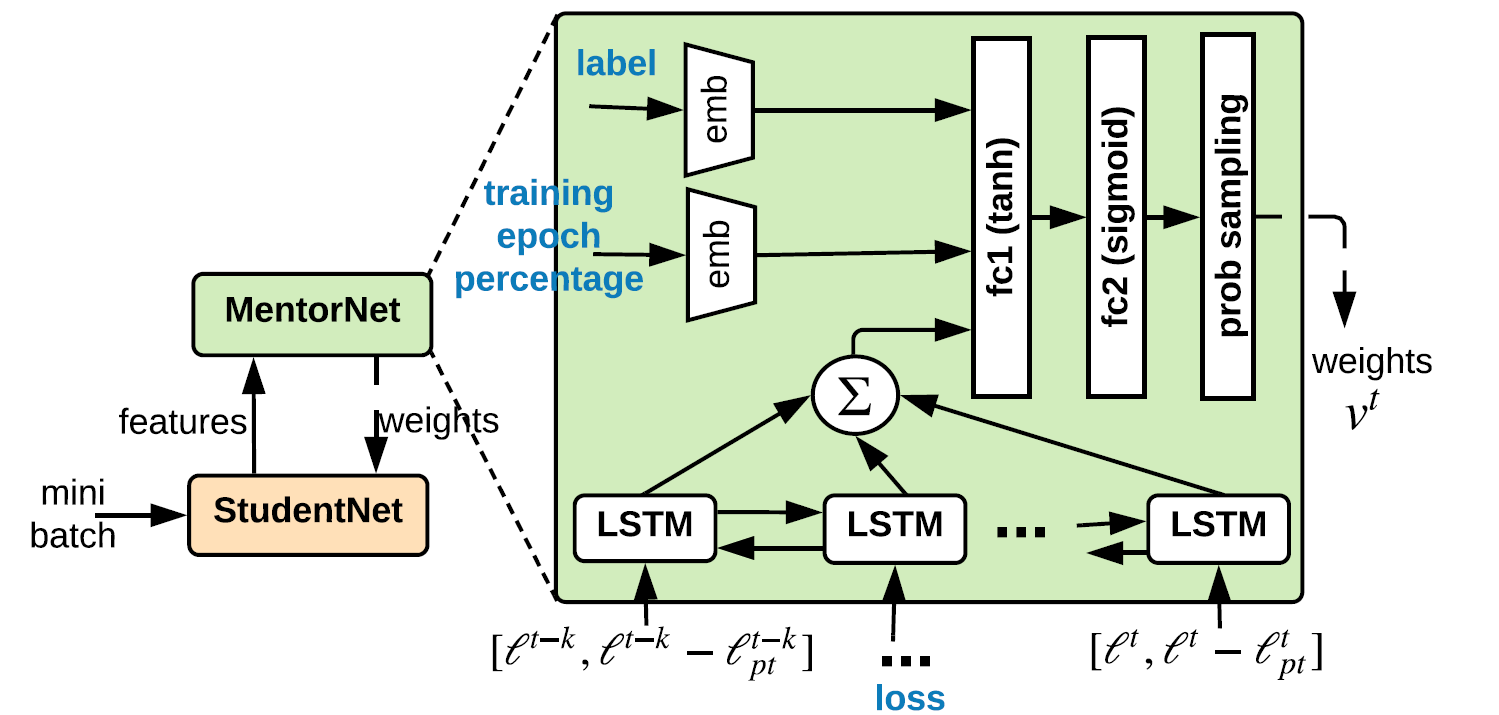
\includegraphics[width=0.9\textwidth]{/images/arch.PNG}
	\caption{from Jiang et al.(2017) MentorNet}
\end{figure}

\subsection{dict look-up}
与上文提到的 memory-bank 方法类似,根据一个样本,通过随机变换得到新样本作为正例,之后取 K 个负例求出 InfoNCE loss 进行优化。不同的是负例的选择方式和编码器的更新方式。

\subsection{Momentum Contrast}
\subsubsection{queue}

每次取得一个新的batch数据进行随机增强作为请求 q,再做另一种随机增强作为每个单独请求的正例 k。将队列中的全部元素作为每个请求的负例,求得损失,利用梯度下降更新参数。随后将 k 加入到队列中,同时去掉旧的batch。
由于队列的规模会很大,队列中的编码加入队列后并不会再更新,但这并不会妨碍一致性的保证,因为它总会把最不一致的编码去除掉。

\subsubsection{Momentum update}

在更新参数时,只对query的编码器参数进行梯度下降,而对key编码器进行如下更新:
$$
\theta_k \leftarrow m\theta_k+(1-m)\theta_q
$$

而在实验中,稍大的 m 得到的结果会更好,这也印证了一致性的重要。

\subsubsection{Pretext Task}

前置任务与 memory-bank 类似。这里作者采用了 ResNet 作为编码器,而作者通过实验发现 BN 对编码的学习起到了消极的作用,而这可能是由于 BN 融合了当前batch的信息,在一定程度上会使模型“走捷径”。

对 BN 的问题,作者提出了 shuffling BN 的方法,也就是在 BN 前先将 sample 进行打乱,求得编码后再复原。

\section{Experiments}

\subsection{training}

数据集采用的是 
\begin{itemize}
	\item ImageNet: 包含约 1 百万张图片,1000 个类别。图片的类别分布均匀
	\item Instagram: 由 Instagram 中得到的约 10 亿张图片。具有长尾分布。
\end{itemize}

这里作者是将特征层冻结,微调线性分类层来验证模型的效果。与众多无监督模型进行比对。

\subsection{findings}

\begin{itemize}
	\item 在微调MoCo时,一些超参数与监督式学习模型相差很大,这表明他们的特征分布有较大的差异
	\item 通过与 end-to-end 和 memory-bank 两种方法的对比可以发现,当字典规模较小时,end-to-end 模型和 MoCo 不相上下,memory-bank 则稍逊风骚;但增大字典规模后,end-to-end 模型则受限于算力,无法计算,其他两个模型都可以持续增加,但 MoCo 则明显胜出许多。说明 MoCo 很大的提升了无监督学习的效果。
	\item 若完全复制query编码器参数,则无法收敛
	\item MoCo 可以很好的作为pre-trained模型进行下游任务的学习。
\end{itemize}

\subsection{conclusion}

MoCo 提供了一种对比学习的框架,在能够使字典尽可能大的同时,还可以保证表征空间的一致性。这是一种非常简洁而有效的方法。

\section{References}

Kaiming He and Haoqi Fan and Yuxin Wu and Saining Xie and Ross Girshick. Momentum Contrast for Unsupervised Visual Representation Learning. \textit{arXiv:1911.05722,2020}

\end{document}          
